\documentclass[11pt,compress,t,notes=noshow, xcolor=table]{beamer}
\usepackage[]{graphicx}\usepackage[]{color}
% maxwidth is the original width if it is less than linewidth
% otherwise use linewidth (to make sure the graphics do not exceed the margin)
\makeatletter
\def\maxwidth{ %
  \ifdim\Gin@nat@width>\linewidth
    \linewidth
  \else
    \Gin@nat@width
  \fi
}
\makeatother

\definecolor{fgcolor}{rgb}{0.345, 0.345, 0.345}
\newcommand{\hlnum}[1]{\textcolor[rgb]{0.686,0.059,0.569}{#1}}%
\newcommand{\hlstr}[1]{\textcolor[rgb]{0.192,0.494,0.8}{#1}}%
\newcommand{\hlcom}[1]{\textcolor[rgb]{0.678,0.584,0.686}{\textit{#1}}}%
\newcommand{\hlopt}[1]{\textcolor[rgb]{0,0,0}{#1}}%
\newcommand{\hlstd}[1]{\textcolor[rgb]{0.345,0.345,0.345}{#1}}%
\newcommand{\hlkwa}[1]{\textcolor[rgb]{0.161,0.373,0.58}{\textbf{#1}}}%
\newcommand{\hlkwb}[1]{\textcolor[rgb]{0.69,0.353,0.396}{#1}}%
\newcommand{\hlkwc}[1]{\textcolor[rgb]{0.333,0.667,0.333}{#1}}%
\newcommand{\hlkwd}[1]{\textcolor[rgb]{0.737,0.353,0.396}{\textbf{#1}}}%
\let\hlipl\hlkwb

\usepackage{framed}
\makeatletter
\newenvironment{kframe}{%
 \def\at@end@of@kframe{}%
 \ifinner\ifhmode%
  \def\at@end@of@kframe{\end{minipage}}%
  \begin{minipage}{\columnwidth}%
 \fi\fi%
 \def\FrameCommand##1{\hskip\@totalleftmargin \hskip-\fboxsep
 \colorbox{shadecolor}{##1}\hskip-\fboxsep
     % There is no \\@totalrightmargin, so:
     \hskip-\linewidth \hskip-\@totalleftmargin \hskip\columnwidth}%
 \MakeFramed {\advance\hsize-\width
   \@totalleftmargin\z@ \linewidth\hsize
   \@setminipage}}%
 {\par\unskip\endMakeFramed%
 \at@end@of@kframe}
\makeatother

\definecolor{shadecolor}{rgb}{.97, .97, .97}
\definecolor{messagecolor}{rgb}{0, 0, 0}
\definecolor{warningcolor}{rgb}{1, 0, 1}
\definecolor{errorcolor}{rgb}{1, 0, 0}
\newenvironment{knitrout}{}{} % an empty environment to be redefined in TeX

\usepackage{alltt}
\newcommand{\SweaveOpts}[1]{}  % do not interfere with LaTeX
\newcommand{\SweaveInput}[1]{} % because they are not real TeX commands
\newcommand{\Sexpr}[1]{}       % will only be parsed by R



\usepackage[english]{babel}
\usepackage[utf8]{inputenc}

\usepackage{dsfont}
\usepackage{verbatim}
\usepackage{amsmath}
\usepackage{amsfonts}
\usepackage{bm}
\usepackage{csquotes}
\usepackage{multirow}
\usepackage{longtable}
\usepackage{booktabs}
\usepackage{enumerate}
\usepackage[absolute,overlay]{textpos}
\usepackage{psfrag}
\usepackage{algorithm}
\usepackage{algpseudocode}
\usepackage{eqnarray}
\usepackage{arydshln}
\usepackage{tabularx}
\usepackage{placeins}
\usepackage{tikz}
\usepackage{setspace}
\usepackage{colortbl}
\usepackage{mathtools}
\usepackage{wrapfig}
\usepackage{bm}
\usetikzlibrary{shapes,arrows,automata,positioning,calc,chains,trees, shadows}
\tikzset{
  %Define standard arrow tip
  >=stealth',
  %Define style for boxes
  punkt/.style={
    rectangle,
    rounded corners,
    draw=black, very thick,
    text width=6.5em,
    minimum height=2em,
    text centered},
  % Define arrow style
  pil/.style={
    ->,
    thick,
    shorten <=2pt,
    shorten >=2pt,}
}
\usepackage{subfig}


% Defines macros and environments
\input{../../style/common.tex}
% \input{common.tex}


%\usetheme{lmu-lecture}
\newcommand{\titlefigure}{figure_man/plot_title_eval_regr.png}
\newcommand{\learninggoals}{
\item Know the definitions of mean squared error (MSE) and mean absolute error (MAE)
\item Understand the connections of MSE and MAE to L2 and L1 loss
\item Know the definitions of $R^2$ and generalized $R^2$}
\usepackage{../../style/lmu-lecture}

\let\code=\texttt
\let\proglang=\textsf

\setkeys{Gin}{width=0.9\textwidth}

\title{Introduction to Machine Learning}
% \author{Bernd Bischl, Christoph Molnar, Daniel Schalk, Fabian Scheipl}
\institute{\href{https://compstat-lmu.github.io/lecture_i2ml/}{compstat-lmu.github.io/lecture\_i2ml}}
\date{}

\setbeamertemplate{frametitle}{\expandafter\uppercase\expandafter\insertframetitle}

\begin{document}

% This file loads R packages, configures knitr options and sets preamble.Rnw as parent file
% IF YOU MODIFY THIS, PLZ ALSO MODIFY setup.Rmd ACCORDINGLY...

% Defines macros and environments
\input{../../latex-math/basic-math.tex}
\input{../../latex-math/basic-ml.tex}

%! includes: regression-losses, evaluation-intro

\lecturechapter{Evaluation: Measures for Regression}
\lecture{Introduction to Machine Learning}

% ------------------------------------------------------------------------------

\begin{vbframe}{Mean Squared Error}

The \textbf{mean squared error (MSE)} computes the mean of squared distances 
between the target variable $y$ and the predicted target $\yh$.

$$
MSE = \meanin (\yi - \yih)^2 \in [0;\infty) \qquad \rightarrow L2 \text{ loss}.
$$

\begin{minipage}[c]{0.33\textwidth}
  \raggedright
  \small
  Outliers with large prediction error heavily influence the MSE, as they 
  enter quadratically.
\end{minipage}%
\begin{minipage}[c]{0.67\textwidth}
  \begin{knitrout}\scriptsize
  \definecolor{shadecolor}{rgb}{0.969, 0.969, 0.969}\color{fgcolor}
  {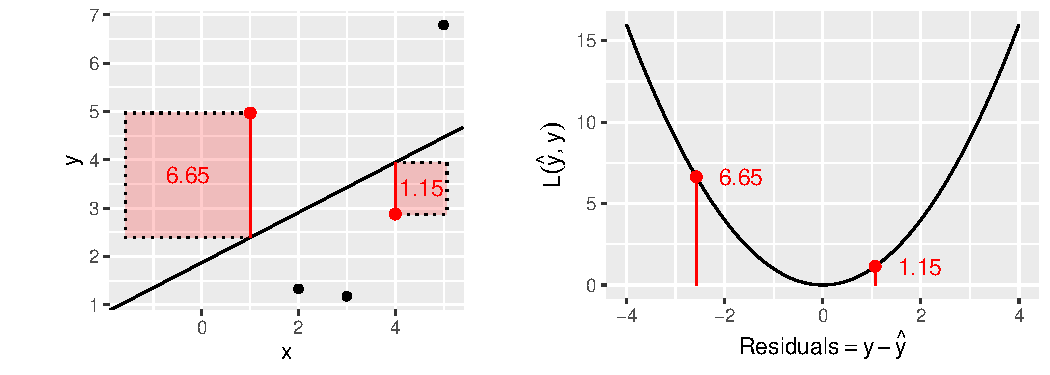
\includegraphics[width=\textwidth]{figure/plot_quad_loss}}
\end{knitrout}
\end{minipage}

% \lz

\small
Similar measures:

\begin{itemize}
  \small
  \item Sum of squared errors (SSE)
  \item Root mean squared error (RMSE) $\rightarrow$ original scale
\end{itemize}

\end{vbframe}

% ------------------------------------------------------------------------------

\begin{vbframe}{Mean Absolute Error}

A more robust (but not necessarily better) alternative is the 
\textbf{mean absolute error (MAE)}:

$$ 
MAE = \meanin \rvert \yi - \yih \rvert \in [0;\infty) \qquad \rightarrow L1 
\text{ loss}.
$$

\begin{minipage}[c]{0.33\textwidth}
  \raggedright
  \small
  The MAE is less strongly impacted by large errors and maybe more 
  intuitive than the MSE.
\end{minipage}%
\begin{minipage}[c]{0.67\textwidth}
  \begin{knitrout}\scriptsize
  \definecolor{shadecolor}{rgb}{0.969, 0.969, 0.969}\color{fgcolor}
  {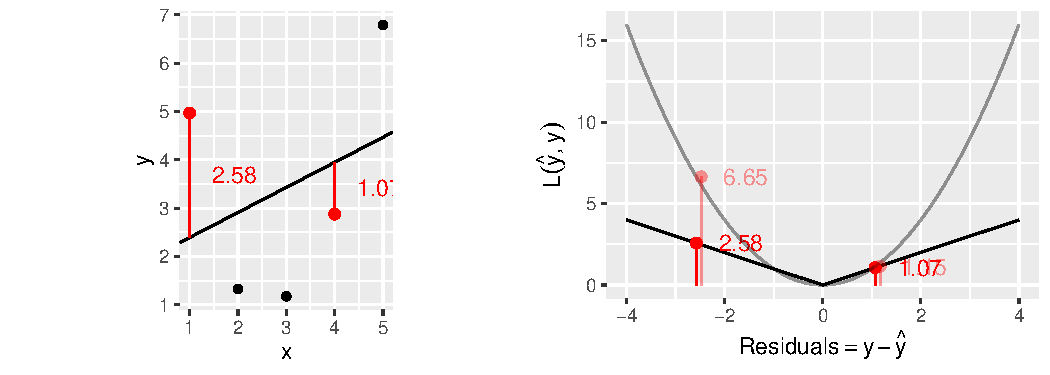
\includegraphics[width=\textwidth]{figure/plot_abs_loss}}
\end{knitrout}
\end{minipage}

\small
Similar measures:

\begin{itemize}
  \small
  \item Median absolute error (for even more robustness)
\end{itemize}

\end{vbframe}

% ------------------------------------------------------------------------------

\begin{vbframe}{$R^2$}
\begin{small}
Another well known measure from statistics is $R^2$:

\[
R^2 = 1 - \frac{\sumin (\yi - \yih)^2}{\sumin (\yi - \bar{y})^2} = 1 - \frac{SSE_{LinMod}}{SSE_{Intercept}}.
\]

\begin{itemize}
  \item Usually introduced as \textbf{fraction of variance explained} by the 
  model.
  \item Simpler explanation: it compares the SSE of a constant model (baseline) 
  to that of a more complex model (LM) on some data, usually the same as used 
  for model fitting.
  \item $R^2=1$: all residuals are 0, we predict perfectly, \\
  $R^2=0$: we predict as badly as the constant model.
  \item If measured on the training data, $R^2 \in [0;1]$, as the LM must be at 
  least as good as the constant, and both SSEs are non-negative.
  \item On other data $R^2$ can even be negative as there is no guarantee that 
  the LM generalizes better than a constant (overfitting).
\end{itemize}
\end{small}
\end{vbframe}

% ------------------------------------------------------------------------------

\begin{vbframe}{Generalized $R^2$ for ML}
A simple generalization of $R^2$ for ML seems to be:

\[
1 - \frac{Loss_{ComplexModel}}{Loss_{SimplerModel}}.
\]

\begin{itemize}
   \item This introduces a general measure of comparison between a simpler 
   baseline and a more complex model considered as an alternative.
  \item Works for arbitrary measures (not only SSE), for arbitrary models, on 
  any data set of interest.
  \item E.g., feature model vs constant, LM vs non-linear model, tree vs forest, 
  model with fewer features vs model with more, ...
  \item In ML we would rather evaluate that metric on a hold-out test set -- 
  there is no reason not to do that.
  \item Fairly unknown; our terminology (generalized $R^2$) is non-standard.
\end{itemize}

\end{vbframe}

% ------------------------------------------------------------------------------

\begin{vbframe}{ml vs classical statistics}

\small

\begin{itemize}
  \item In classical statistics, besides MSE, RMSE and in-sample $R^2$, other 
  metrics are used to evaluate and select regression models. 
  \item They often focus on goodness-of-fit, as measured by (log-)likelihood, 
  rather than predictive accuracy -- for example, information criteria:
  % \item Frequently used metrics are so-called information criteria (lower values 
  % indicating better models): 
  \begin{itemize}
    \small
    \item \textbf{Akaike’s information criterion (AIC)} balances model fit and
    complexity, penalizing the number of parameters, $p$: 
    $$ AIC = -2 \cdot \llt + 2 \cdot p.$$
    
    %\item \textbf{AICc} is a corrected version for AIC for small sample sizes.
    
    \item \textbf{Bayesian information criterion (BIC)} is another variant of 
    the AIC with a stronger penalty for more complex models: 
    $$ BIC = -2 \cdot \llt + \log(p).$$
  \end{itemize}
    
  % \item By adding the number of parameters $p$ to the evaluation metric, more 
  % complex models are penalized. 
    
  \item As both AIC and BIC are based upon a ground-truth distribution, they 
  cannot be used to compare performances across different data sets.
  \item NB: using the same data for training and evaluation / model selection 
  introduces optimistic bias $\rightarrow$ post-selection inference.
    
 \end{itemize}

\end{vbframe}

% ------------------------------------------------------------------------------

\endlecture
\end{document}